\section*{Assignment 5}
% Password.
% Fpga was counting time ow long the responsetime was for responding, waiting for the 1st didgit of the answere. middelng the time between als answeres to get the longes one right. using thatone as correct didgit of the PW.
%
% building the counter 4 the clockcycles was the hard part strings where to long
% fpga giving back the time  we had to use 2 bytes
% 
% python did the rest.

Like in assignment 4, we get a microcontroller (we know, that its sowftware is written using the c programming language) and analyse it the same way as before. 
This time it directly prompts \textit{``Please enter password:''}, answering \textit{``Password incorrect''} to our guesses and the goal is set. As a possible attack vector comes a timing vulnerability to mind, if the password comparison is implemented using \texttt{strcmp}. We continue setting up the FPGA like before -- able to reset the device on command and relaying all communication. We just need a little further testing to be sure, that we are indeed going to program a timing attack.

To measure the timing of the string comparison on the micro controller, we have to know when it is actually executed, or, in other words how long it takes the device to send \textit{``Please enter password:''} leading to it being in a state, where it excepts input. 
Again we use an oscilloscope hooked to the \texttt{tx} line of the device to obtain this timing offset. 

Remember, at this point the FPGA is already set up like in figure \ref{fig:as4-schematic-1} (p.~\pageref{fig:as4-schematic-1}).
We add another receiver (to whats comming from the device), and a transmitter (to the computer), tell the FPGA in a finite 3-state machine to start the timer on receiving `:', stop it on receiving `i', and transmit the measurement to the computer afterwards, as shown in figure \ref{fig:as5-schematic} (p.~\pageref{fig:as5-schematic}). Technically, that is achieved by counting the clock cycles between both events in a 2 byte integer; if the FPGA is relaying the micro controllers output, or sending the measured timing is determined by a multiplexer.

Now a Python script can launch the attack, bruteforcing every single sign at a time, again:

\begin{enumerate}
    \item Wait the timing offset;
    \item transmit the current password guess;
    \item receive 2 bytes timing score;
    \item add the sign with the highest timing score to the known password.
\end{enumerate}

We actually take several measurements for every password guess and take the mean in order to be less error-prone.


\begin{figure}[h!]
    \begin{center}
%        \hrule\vspace{1em}
        \usetikzlibrary{arrows.meta}
\usetikzlibrary{calc,intersections,through,backgrounds}
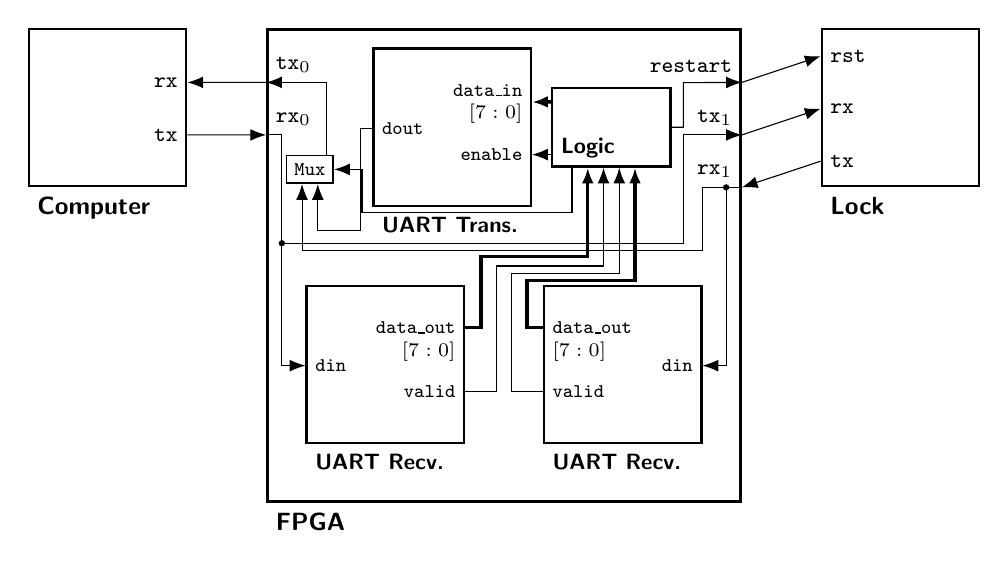
\begin{tikzpicture}
% 	\tikzset{
% 	  every node/.style={scale=1.1}
% 	}	
	\tikzset{comp/.style={
		rectangle, draw=black, thick
	}}	
	\tikzset{component/.style={
		comp, minimum width=6cm, minimum height=6cm, very thick
	}}
	\tikzset{component_small/.style={
		comp, minimum width=2cm, minimum height=2cm, thick
	}}
	\tikzset{component_tiny/.style={
		comp, inner sep=0.1cm, semithick, right
	}}
	\tikzset{caption/.style={
		below right
	}}
	\tikzset{conn/.style={
		-{Latex[length=2mm]}
	}}
	
	% FPGA
	\node (FPGA) [component] at (0,0) {}
		% Caption
		node [caption] at (FPGA.south west) { \small{\textsf{\textbf{FPGA}}} }
		
		% In/-outputs links
		coordinate [yshift=4cm+0.4pt+0.666cm, label={ above right : \footnotesize{$\texttt{rx}_0$} }] (FPGA_rx0) at (FPGA.south west) % unten
		coordinate [yshift=4cm+0.4pt+1.333cm, label={ above right : \footnotesize{$\texttt{tx}_0$} }] (FPGA_tx0) at (FPGA.south west) % oben

		% In/outputs  rechts
		coordinate [yshift=4cm+0.4pt,                    label={ above left : \footnotesize{$\texttt{rx}_1$} }]      (FPGA_rx1)       at (FPGA.south east)  % unten
		coordinate [yshift=4cm+0.4pt+0.666cm, label={ above left : \footnotesize{$\texttt{tx}_1$} }]      (FPGA_tx1)       at (FPGA.south east) % mitte
		coordinate [yshift=4cm+0.4pt+1.333cm, label={ above left : \footnotesize{$\texttt{restart}$} }] (FPGA_restart) at (FPGA.south east) % oben
		
		% Internals
		node (Mux)          [component_tiny, shift={(0.25cm,-1.8cm) }]  at (FPGA.north west)   { \scriptsize{\textsf{\texttt{Mux}}} }
	;

	% Logic
	\node (Logic) at (FPGA.north) [comp, minimum height=1cm, minimum width=1.5cm, below right, shift={(0.6cm, -0.75cm)}] {}
		node [above right] at (Logic.south west) { \textsf{\footnotesize{\textbf{Logic}}} }
	;

	% Receiver
	\node (Receiver) at (FPGA.south east) [component_small, above left, shift={(-0.5, 0.75)}] {}
		% Caption
		node [caption] at (Receiver.south west) { \textsf{\footnotesize{\textbf{UART Recv.}}} }

		% Input rechts
		coordinate [yshift=1cm, label={ left : \scriptsize{\texttt{din}} }] (Receiver_din) at (Receiver.south east)

		% Outpus links
		coordinate [yshift=0.666cm,                 label={ right : \scriptsize{\texttt{valid}} }]           (Receiver_valid)           at (Receiver.south west) % unten
		coordinate [yshift=1.333cm+0.15cm, label={ right : \scriptsize{\texttt{data\_out}} }] (Receiver_data_out)    at (Receiver.south west) % oben
		coordinate [yshift=1.333cm-0.15cm,  label={ right : \scriptsize{$[7:0]$} }]                     (Receiver_data_out2) at (Receiver.south west) % mitte
	;

	% Receiver2
	\node (Receiver2) at (FPGA.south west) [component_small, above right, shift={(0.5, 0.75)}] {}
		% Caption
		node [caption] at (Receiver2.south west) { \textsf{\footnotesize{\textbf{UART Recv.}}} }

		% Input rechts
		coordinate [yshift=1cm, label={ right : \scriptsize{\texttt{din}} }] (Receiver2_din) at (Receiver2.south west)

		% Outpus links
		coordinate [yshift=0.666cm,                 label={ left : \scriptsize{\texttt{valid}} }]           (Receiver2_valid)           at (Receiver2.south east) % unten
		coordinate [yshift=1.333cm+0.15cm, label={ left : \scriptsize{\texttt{data\_out}} }] (Receiver2_data_out)    at (Receiver2.south east) % oben
		coordinate [yshift=1.333cm-0.15cm,  label={ left : \scriptsize{$[7:0]$} }]                     (Receiver2_data_out2) at (Receiver2.south east) % mitte
	;

	% Transmitter
	\node (Transmitter) at (FPGA.north west) [component_small, below right, shift={(1.35, -0.25)}] {}
		node [caption] at (Transmitter.south west) { \textsf{\footnotesize{\textbf{UART Trans.}}} }

		% Output links
		coordinate [yshift=1cm, label={ right: \scriptsize{\textsf{\texttt{dout}}} }] (Transmitter_dout) at (Transmitter.south west) % unten

		% Inputs links
		coordinate [yshift=0.666cm,                 label={ left : \scriptsize{\texttt{enable}} }]    (Transmitter_enable)   at (Transmitter.south east) % unten
		coordinate [yshift=1.333cm-0.15cm,  label={ left : \scriptsize{$[7:0]$} }]                  (Transmitter_data_in2)at (Transmitter.south east) % mitte
		coordinate [yshift=1.333cm+0.15cm, label={ left : \scriptsize{\texttt{data\_in}} }] (Transmitter_data_in)  at (Transmitter.south east) % oben	
	;

	% Computer
	\node (Computer) [component_small, below left, xshift=-1cm] at (FPGA.north west) {}
		% Caption
		node [caption] at (Computer.south west) { \small{\textsf{\textbf{Computer}}} }

		% In/outputs rechts
		coordinate [yshift=0.666cm, label={ left:\footnotesize{\texttt{tx}} }] (Computer_tx) at (Computer.south east) % unten
		coordinate [yshift=1.333cm, label={ left:\footnotesize{\texttt{rx}} }] (Computer_rx) at (Computer.south east) % oben
	;

	% Lock
	\node (Lock) [component_small, below right, xshift=1cm] at (FPGA.north east) {}
		% Caption
		node [caption] at (Lock.south west) { \small{\textsf{\textbf{Lock}}} }

		% In/outputs rechts
		coordinate [yshift=0.333cm, label={ right:\footnotesize{\texttt{tx}} }]   (Lock_tx)   at (Lock.south west) % unten
		coordinate [yshift=0.999cm, label={ right:\footnotesize{\texttt{rx}} }]   (Lock_rx)   at (Lock.south west) % mitte
		coordinate [yshift=1.666cm, label={ right:\footnotesize{\texttt{rst}} }] (Lock_rst)  at (Lock.south west) % oben
	;

	% Computer <-> FPGA
	\draw[conn]  (FPGA_tx0) -- (Computer_rx);
	\draw[conn] (Computer_tx) -- (FPGA_rx0);

	% FPGA <-> Lock
	\draw[conn] (FPGA_restart) -- (Lock_rst);
	\draw[conn] (FPGA_tx1) -- (Lock_rx);
	\draw[conn] (Lock_tx) -- (FPGA_rx1) ;
	
	% FPGA internal
		\draw[conn] (Logic.east) -| ([shift={(0.15cm, 0.566cm)}] Logic.east) -- (FPGA_restart);
		\draw[conn, name path=FPGA_rx0--FPGA_tx1] (FPGA_rx0) -| ([shift={(0.2cm, -1.375cm)}] FPGA_rx0) -- ([shift={(5.3cm, -1.375cm)}] FPGA_rx0) |- (FPGA_tx1); % Pass through Computer -> Lock
	
		% Connections to/from Receiver
		\draw[conn, name path=FPGA_rx1--Receiver_din] (FPGA_rx1) -- ([xshift=-0.2cm] FPGA_rx1) |- (Receiver_din); % rx1 -> Logic
		\draw[conn, very thick] (Receiver_data_out) -|  ([shift={(-0.2cm,0.6cm)}] Receiver_data_out) -| ([xshift=0.3cm] Logic.south);  % data_out -> Logic
		\draw[conn] (Receiver_valid) -| ([shift={(-0.4cm, 1.5cm)}] Receiver_valid) -| ([xshift=0.1cm] Logic.south); % valid -> Logic
		
		% Connections to/from Receiver2
		\draw[conn, name path=FPGA_rx0--Receiver2_din] (FPGA_rx0) -- ([xshift=0.2cm] FPGA_rx0) |- (Receiver2_din); % rx0 -> din
		\draw[conn, very thick] (Receiver2_data_out) -| ([shift={(0.2cm,0.9cm)}] Receiver2_data_out) -| ([xshift=-0.3cm] Logic.south); % data_out -> Logic 
		\draw[conn] (Receiver2_valid) -| ([shift={(0.4cm, 1.6cm)}] Receiver2_valid) -| ([xshift=-0.1cm] Logic.south); % valid -> Logic

		% Connections to/from Transmitter
		\draw[conn, very thick] ([yshift=-0.192cm] Logic.north west) -- ([yshift=-0.15cm] Transmitter_data_in); % Logic -> data_in
		\draw[conn] ([yshift=0.166cm] Logic.south west) -- (Transmitter_enable); % Logic -> enable
		\draw[conn] (Transmitter_dout) -| ([shift={(-0.15cm, -1.3cm)}] Transmitter_dout) -| ([xshift=0.1cm] Mux.south); % Transmitter -> Mux

		% Connections to/from Mux
		\draw[conn, name path=FPGA_rx1--Mux]  (FPGA_rx1) -- ([xshift=-0.5cm] FPGA_rx1) |-  ([shift={(-0.2cm, -1.55cm)}]  Transmitter_dout) -| ([xshift=-0.1cm] Mux.south); % rx1 -> Mux
		\draw[conn] ([xshift=-0.5cm] Logic.south) |- ([shift={(0.355cm, -0.55cm)}] Mux.east) |- (Mux.east); % Logic -> Mux
		\draw[conn] ([xshift=-0.1cm] Mux.north east) |- (FPGA_tx0); % Mux -> tx0

		% Intersections
		\fill[name intersections={of=FPGA_rx0--FPGA_tx1 and FPGA_rx0--Receiver2_din, total=\t}] (intersection-\t) circle (0.4mm);
		\fill[name intersections={of=FPGA_rx1--Mux and FPGA_rx1--Receiver_din, total=\t}] (intersection-\t) circle (0.4mm);
\end{tikzpicture}
        \caption{Timing attack.}
        \label{fig:as5-schematic}
        \vspace{1em}\hrule
    \end{center}
\end{figure}
